\chapter{Specifikacija programske potpore}
		
	\section{Funkcionalni zahtjevi}
			
			\noindent \textbf{Dionici:}
			
			\begin{packed_enum}
				
				\item Korisnici			
				\begin{packed_enum}
					
					\item Polaznik
					\item Predavač	
				\end{packed_enum}
				\item Administrator			
				\item Razvojni tim
				
			\end{packed_enum}
			
			\noindent \textbf{Aktori i njihovi funkcionalni zahtjevi:}
			
			
			\begin{packed_enum}
				\item  \underbar{Neregistrirani korisnik (inicijator) može:}
				
				\begin{packed_enum}
					
					\item registrirati se u sustav
					\begin{packed_enum}
						
						\item  stvoriti novi korisnički račun polaznika za koji su mu potrebni korisničko ime, lozinka, ime, prezime, e-mail adresa i broj kartice za naplatu \textbf{ili}
						\item  stvoriti novi korisnički račun predavača za koji su mu potrebni korisničko ime, lozinka, ime, prezime, e-mail adresa i IBAN računa, uz opciju stavljanja svoje slike i kratke biografije
				
					\end{packed_enum}
	
				\end{packed_enum}
			
				\item  \underbar{Predavač (inicijator) može:}
				
				\begin{packed_enum}
					
					\item pregledavati i mijenjati osobne podatke
					\item pretraživati ponuđene tečajeve
					\item dodati, urediti i obrisati tečaj
					\item pregledati polaznike svojih tečajeva
					\item pregledati i odgovoriti na recenzije
					\item prihvatiti ili odbiti termin konzultacija
					
				\end{packed_enum}
			
			\eject
			
				\item  \underbar{Polaznik (inicijator) može:}
				
				\begin{packed_enum}
					
					\item pregledavati i mijenjati osobne podatke
					\item pretraživati ponuđene tečajeve
					\item upisati i platiti tečaj
					\item pristupiti plaćenom tečaju
					\item preuzimati materijale upisanog tečaja
					\item poslati zahtjev za konzultacijama
					\item pregledati recenzije svih tečajeva
					\item objaviti recenziju na upisanom tečaju
					
				\end{packed_enum}
			
				\item  \underbar{Administrator (inicijator) može:}
				
				\begin{packed_enum}
					
					\item vidjeti popis svih registriranih korisnika aplikacije
					\item brisati korisnike
					\item urediti i obrisati tečaj
					\item dodati i obrisati kategoriju tečaja
					\item pregledati i odgovoriti na recenzije
					\item obrisati recenzije koje su u suprotnosti s pravilima korištenja aplikacije
					\item pristupiti statistici
					
				\end{packed_enum}
			
				\item  \underbar{Baza podataka (sudionik):}
				
				\begin{packed_enum}
					
					\item pohranjuje sve podatke o korisnicima
					\item pohranjuje sve podatke o tečajevima i njihove materijale
					
				\end{packed_enum}
			\end{packed_enum}
			
			\eject 
			
			
				
			\subsection{Obrasci uporabe}
				
				
				\subsubsection{Opis obrazaca uporabe}

					\noindent \underbar{\textbf{UC1 - Registracija}}
					\begin{packed_item}
	
						\item \textbf{Glavni sudionik:} Korisnik
						\item  \textbf{Cilj:} Izbor maila i korisničke adrese
						\item  \textbf{Sudionici:} Baza podataka
						\item  \textbf{Preduvjet:} -
						\item  \textbf{Opis osnovnog tijeka:}
						
						\item[] \begin{packed_enum}
	
							\item Korisnik unosi potrebne podatke
							\item Korisnik je usmjeren na stranicu za unos dodatnih podataka (\hyperref[UC2] {UC2})
							
						\end{packed_enum}
						
						\item  \textbf{Opis mogućih odstupanja:}
						
						\item[] \begin{packed_item}
	
							\item[1.a] Odabir već zauzetog korisničkog imena i/ili e-maila, unos korisničkog podatka u nedozvoljenom formatu ili pružanje neispravnog e-maila
							\item[] \begin{packed_enum}
								
								\item Sustav obavještava korisnika o neuspjelom upisu i vraća ga na stranicu za registraciju
								
							\end{packed_enum}
							
						\end{packed_item}
					\end{packed_item}
									
					\noindent \label{UC2} \underbar{\textbf{UC2 - Unos podataka}}
					\begin{packed_item}
						
						\item \textbf{Glavni sudionik:} Korisnik
						\item  \textbf{Cilj:} Stvoriti korisnički račun za pristup sustavu
						\item  \textbf{Sudionici:} Baza podataka
						\item  \textbf{Preduvjet:} Uspješan unos e-mail adrese i korisničkog imena
						\item  \textbf{Opis osnovnog tijeka:}
						
						\item[] \begin{packed_enum}
							
							\item Korisnik unosi potrebne podatke
							\item Korisnik prima obavijest o uspješnoj registraciji
							
						\end{packed_enum}
						
						\item  \textbf{Opis mogućih odstupanja:}
						
						\item[] \begin{packed_item}
							
							\item[1.a] Ostavljen prazan jedan od potrebnih podataka
							\item[] \begin{packed_enum}
								
								\item Sustav obavještava korisnika da mora unijeti podatak
								
							\end{packed_enum}
							\item[1.b] Korisnik odustaje od registracije
							\item[] \begin{packed_enum}
								
								\item Sustav briše cijelu registraciju
								
							\end{packed_enum}
							
						\end{packed_item}
					\end{packed_item}
			
					\noindent \underbar{\textbf{UC3 - Prijava}}
					\begin{packed_item}
						
						\item \textbf{Glavni sudionik:} Korisnik
						\item  \textbf{Cilj:} Pristup sustavu
						\item  \textbf{Sudionici:} Baza podataka
						\item  \textbf{Preduvjet:} Postojeći račun u sustavu
						\item  \textbf{Opis osnovnog tijeka:}
						
						\item[] \begin{packed_enum}
							
							\item Korisnik unosi e-mail i šifru
							\item Korisnik prima obavijest o uspješnoj prijavi
							
						\end{packed_enum}
						
						\item  \textbf{Opis mogućih odstupanja:}
						
						\item[] \begin{packed_item}
							
							\item[1.a] Ostavljen prazan jedan od potrebnih podataka
							\item[] \begin{packed_enum}
								
								\item Sustav obavještava korisnika da mora unijeti podatak
								
							\end{packed_enum}
							\item[1.b] Unesen krivi e-mail ili šifra
							\item[] \begin{packed_enum}
								
								\item Sustav obavještava korisnika o neispravnosti unesenih podataka
								
							\end{packed_enum}
							
						\end{packed_item}
					\end{packed_item}
		
				\noindent \underbar{\textbf{UC4 - Pregled tečajeva}}
				\begin{packed_item}
					
					\item \textbf{Glavni sudionik:} Polaznik, Predavač, Administrator
					\item  \textbf{Cilj:} Uspješan prikaz dostupnih tečajeva
					\item  \textbf{Sudionici:} Baza podataka
					\item  \textbf{Preduvjet:} Uspješna prijava
					\item  \textbf{Opis osnovnog tijeka:}
					
					\item[] \begin{packed_enum}
						
						\item Tečajevi su prikazani na aplikaciji
						
					\end{packed_enum}
					
				\end{packed_item}
			
				\noindent \underbar{\textbf{UC5 - Pristup tečaju}}
				\begin{packed_item}
					
					\item \textbf{Glavni sudionik:} Polaznik, Administrator
					\item  \textbf{Cilj:} Pristup sadržaju tečaja
					\item  \textbf{Sudionici:} Baza podataka
					\item  \textbf{Preduvjet:} Uspješna prijava i plaćen tečaj kojem se pristupa ili dodijeljena prava administratora
					\item  \textbf{Opis osnovnog tijeka:}
					
					\item[] \begin{packed_enum}
						
						\item Polaznik odabire tečaj
						\item Polaznik je usmjeren na stranicu tečaja
						
					\end{packed_enum}
					
				\end{packed_item}
				\noindent \underbar{\textbf{UC6 - Upis tečaja}}
				\begin{packed_item}
					
					\item \textbf{Glavni sudionik:} Polaznik
					\item  \textbf{Cilj:} Dobivanje pristupa tečaju
					\item  \textbf{Sudionici:} Baza podataka
					\item  \textbf{Preduvjet:} Uspješna prijava i tečaj kojeg polaznik nije još platio
					\item  \textbf{Opis osnovnog tijeka:}
					
					\item[] \begin{packed_enum}
						
						\item Polaznik odabire željeni tečaj
						\item Polaznik je usmjeren na stranicu za naplatu tečaja
						
					\end{packed_enum}
					
				\end{packed_item}
			
				\noindent \underbar{\textbf{UC7 - Naplata tečaja}}
				\begin{packed_item}
					
					\item \textbf{Glavni sudionik:} Polaznik
					\item  \textbf{Cilj:} Uspješna naplata tečaja
					\item  \textbf{Sudionici:} Baza podataka
					\item  \textbf{Preduvjet:} Uspješna prijava
					\item  \textbf{Opis osnovnog tijeka:}
					
					\item[] \begin{packed_enum}
						
						\item Polaznik potvrđuje odabrani tečaj i iznos naplate
						\item Polaznik izvršava plaćanje tečaja
						
					\end{packed_enum}
					
					\item  \textbf{Opis mogućih odstupanja:}
					
					\item[] \begin{packed_item}
						
						\item[2.a] Nedovoljno sredstava na kartici
						\item[] \begin{packed_enum}
							
							\item Sustav obavještava polaznika o nemogućnosti pohađanja tečaja zbog financija
							
						\end{packed_enum}
						
					\end{packed_item}
				\end{packed_item}
			
				\noindent \underbar{\textbf{UC8 - Dodavanje tečaja}}
				\begin{packed_item}
					
					\item \textbf{Glavni sudionik:} Predavač
					\item  \textbf{Cilj:} Uspješno kreiranje tečaja
					\item  \textbf{Sudionici:} Baza podataka
					\item  \textbf{Preduvjet:} Uspješna prijava
					\item  \textbf{Opis osnovnog tijeka:}
					
					\item[] \begin{packed_enum}
						
						\item Predavač unosi potrebne podatke o tečaju
						\item Predavač dodaje materijale za tečaj
						
					\end{packed_enum}
					
				\end{packed_item}
			
			\noindent \underbar{\textbf{UC9 - Brisanje tečaja}}
			\begin{packed_item}
				
				\item \textbf{Glavni sudionik:} Predavač, Administrator
				\item  \textbf{Cilj:} Uspješno ukloniti tečaj
				\item  \textbf{Sudionici:} Baza podataka
				\item  \textbf{Preduvjet:} Uspješna prijava i vlasništvo tečaja ili dodijeljena prava administratora
				\item  \textbf{Opis osnovnog tijeka:}
				
				\item[] \begin{packed_enum}
					
					\item Predavač izabire brisanje vlastitog tečaja
					\item Predavač potvrđuje brisanje tečaja
					\item Tečaj je uklonjen iz baze podataka
					
				\end{packed_enum}
				\item  \textbf{Opis mogućih odstupanja:}
				
				\item[] \begin{packed_item}
					
					\item[1.a] Postoje zahtjevi za konzultacijama na tom tečaju
					\item[] \begin{packed_enum}
						
						\item Sustav otkazuje sve konzultacije
						
					\end{packed_enum}
					
				\end{packed_item}
				
			\end{packed_item}
				
			\noindent \underbar{\textbf{UC10 - Uređivanje tečaja}}
			\begin{packed_item}
				
				\item \textbf{Glavni sudionik:} Predavač, Administrator
				\item  \textbf{Cilj:} Promjena opisa i/ili materijala tečaja
				\item  \textbf{Sudionici:} Baza podataka
				\item  \textbf{Preduvjet:} Uspješna prijava i vlasništvo tečaja ili dodijeljena prava administratora
 				\item  \textbf{Opis osnovnog tijeka:}
				
				\item[] \begin{packed_enum}
					
					\item Predavač izabire uređivanje vlastitog tečaja
					\item Predavač mijenja sadržaj tečaja i/ili materijala
					
				\end{packed_enum}
				
			\end{packed_item}	
		
			\noindent \underbar{\textbf{UC11 - Objava recenzije}}
			\begin{packed_item}
				
				\item \textbf{Glavni sudionik:} Polaznik
				\item  \textbf{Cilj:} Objava recenzije na stranici tečaja i profilu predavača
				\item  \textbf{Sudionici:} Baza podataka
				\item  \textbf{Preduvjet:} Uspješna prijava i plaćen tečaj na kojem se recenzija objavljuje
				\item  \textbf{Opis osnovnog tijeka:}
				
				\item[] \begin{packed_enum}
					
					\item Polaznik unosi recenziju
					\item Recenzija se dodaje na stranicu tečaja
					
				\end{packed_enum}
				
			\end{packed_item}
		
			\noindent \underbar{\textbf{UC12 - Pregled recenzija}}
			\begin{packed_item}
				
				\item \textbf{Glavni sudionik:} Predavač, Administrator, Polaznik
				\item  \textbf{Cilj:} Pregled recenzija
				\item  \textbf{Sudionici:} Baza podataka
				\item  \textbf{Preduvjet:} Uspješna prijava
				\item  \textbf{Opis osnovnog tijeka:}
				
				\item[] \begin{packed_enum}
					
					\item Prikaz recenzije odabranog predavača ili tečaja
					
				\end{packed_enum}
				
			\end{packed_item}
		
			\noindent \underbar{\textbf{UC13 - Odgovaranje na recenziju}}
			\begin{packed_item}
				
				\item \textbf{Glavni sudionik:} Predavač, Administrator
				\item  \textbf{Cilj:} Objava odgovora na recenziju
				\item  \textbf{Sudionici:} Baza podataka
				\item  \textbf{Preduvjet:} Uspješna prijava i vlasništvo tečaja ili dodijeljena prava administratora
				\item  \textbf{Opis osnovnog tijeka:}
				
				\item[] \begin{packed_enum}
					
					\item Predavač odabire recenziju na koju želi odgovoriti
					\item Predavač objavljuje svoj odgovor na željenu recenziju
					
				\end{packed_enum}
			
			\end{packed_item}
			\noindent \underbar{\textbf{UC14 - Brisanje recenzije}}
			\begin{packed_item}
				
				\item \textbf{Glavni sudionik:} Administrator
				\item  \textbf{Cilj:} Uklanjanje recenzije sa stranice tečaja ili profila predavača
				\item  \textbf{Sudionici:} Baza podataka
				\item  \textbf{Preduvjet:} Korisnik je registriran i dodijeljena su mu prava administratora
				\item  \textbf{Opis osnovnog tijeka:}
				
				\item[] \begin{packed_enum}
					
					\item Odabir recenzije koju je potrebno ukloniti
					\item Uklanjanje recenzije sa stranice tečaja ili profila predavača
					
				\end{packed_enum}

			\end{packed_item}
		
			\noindent \label{UC15} \underbar{\textbf{UC15 - Slanje zahtjeva za konzultacijama}}
			\begin{packed_item}
				
				\item \textbf{Glavni sudionik:} Polaznik
				\item  \textbf{Cilj:} Uspješno poslati zahtjev za terminom
				\item  \textbf{Sudionici:} Baza podataka
				\item  \textbf{Preduvjet:} Uspješna prijava i plaćen tečaj za kojeg se traže konzultacije
				\item  \textbf{Opis osnovnog tijeka:}
				
				\item[] \begin{packed_enum}
					
					\item Odabir tečaja za kojeg se traže konzultacije
					\item Odabir termina za konzultacije
					
				\end{packed_enum}
				
			\end{packed_item}
		
			\noindent \underbar{\textbf{UC16 - Odgovor na zahtjev za terminom konzultacija}}
			\begin{packed_item}
				
				\item \textbf{Glavni sudionik:} Predavač
				\item  \textbf{Cilj:} Odgovoriti na zahtjev za terminom konzultacija
				\item  \textbf{Sudionici:} Baza podataka
				\item  \textbf{Preduvjet:} Uspješna prijava i vlasništvo tečaja
				\item  \textbf{Opis osnovnog tijeka:}
				
				\item[] \begin{packed_enum}
					
					\item Odobravanje primljenog zahtjeva za terminom konzultacija 
					\item Polaznik dobiva obavijest o potvrđenom terminu
					
				\end{packed_enum}
				\textbf{ili}
			
				\item[] \begin{packed_enum}
					
					\item Odbijanje termina konzultacija
					\item Polaznik prima obavijest o odbijenom terminu
					\item Polaznik traži novi termin \hyperref[UC15]{(UC15)}
					
				\end{packed_enum}
				
			\end{packed_item}
		
		
			\noindent \underbar{\textbf{UC17 - Brisanje korisnika}}
			\begin{packed_item}
				
				\item \textbf{Glavni sudionik:} Administrator
				\item  \textbf{Cilj:} Uspješno ukloniti korisnika iz sustava
				\item  \textbf{Sudionici:} Baza podataka
				\item  \textbf{Preduvjet:} Korisnik je registriran i dodijeljena su mu prava administratora
				\item  \textbf{Opis osnovnog tijeka:}
				
				\item[] \begin{packed_enum}
					
					\item Odabir korisnika čiji se račun uklanja
					\item Ukoliko je korisnik predavač, sustav uklanja njegov profil i sve njegove tečajeve iz baze podataka. Ukoliko je korisnik polaznik, sustav ga uklanja s upisanih tečajeva te njegov profil iz baze podataka
					
				\end{packed_enum}
				
			\end{packed_item}
		
			\noindent \underbar{\textbf{UC18 - Pregled statistike}}
			\begin{packed_item}
				
				\item \textbf{Glavni sudionik:} Administrator
				\item  \textbf{Cilj:} Uspješno prikazati statistiku korisnika na aplikaciji
				\item  \textbf{Sudionici:} Baza podataka
				\item  \textbf{Preduvjet:} Korisnik je registriran i dodijeljena su mu prava administratora
				\item  \textbf{Opis osnovnog tijeka:}
				
				\item[] \begin{packed_enum}
					
					\item Prikaz statistike korištenja aplikacije i statistike njenih korisnika
					
				\end{packed_enum}
				
			\end{packed_item}
		
			\noindent \underbar{\textbf{UC19 - Dodavanje kategorije}}
			\begin{packed_item}
				
				\item \textbf{Glavni sudionik:} Administrator
				\item  \textbf{Cilj:} Uspješno dodana nova kategorija tečajeva
				\item  \textbf{Sudionici:} Baza podataka
				\item  \textbf{Preduvjet:} Korisnik je registriran i dodijeljena su mu prava administratora
				\item  \textbf{Opis osnovnog tijeka:}
				
				\item[] \begin{packed_enum}
					
					\item Unos podataka o kategoriji tečaja
					\item Unos mogućih razina kategorije tečaja
					
				\end{packed_enum}
				
			\end{packed_item}
		
			\noindent \underbar{\textbf{UC20 - Brisanje kategorije}}
			\begin{packed_item}
				
				\item \textbf{Glavni sudionik:} Administrator
				\item  \textbf{Cilj:} Uspješno ukloniti kategoriju tečaja
				\item  \textbf{Sudionici:} Baza podataka
				\item  \textbf{Preduvjet:} Korisnik je registriran i dodijeljena su mu prava administratora
				\item  \textbf{Opis osnovnog tijeka:}
				
				\item[] \begin{packed_enum}
					
					\item Odabir kategorije koju se želi ukloniti
					\item Svi tečajevi pod odabranom kategorijom uklonjeni iz baze podataka
					\item Kategorija je uklonjena iz baze podataka
					
				\end{packed_enum}
				
			\end{packed_item}
		
		
			\noindent \underbar{\textbf{UC21 - Pregled korisnika}}
			\begin{packed_item}
				
				\item \textbf{Glavni sudionik:} Administrator
				\item  \textbf{Cilj:} Uspješno dohvatiti popis korisnika aplikacije
				\item  \textbf{Sudionici:} Baza podataka
				\item  \textbf{Preduvjet:} Korisnik je registriran i dodijeljena su mu prava administratora
				\item  \textbf{Opis osnovnog tijeka:}
				
				\item[] \begin{packed_enum}
					
					\item Odabir prikaza popisa korisnika aplikacije
					
				\end{packed_enum}
				
			\end{packed_item}
			\noindent \label{UC22} \underbar{\textbf{UC22 - Pregled osobnih podataka}}
			\begin{packed_item}
				
				\item \textbf{Glavni sudionik:} Predavač, Polaznik
				\item  \textbf{Cilj:} Pregledati osobne podatke
				\item  \textbf{Sudionici:} Baza podataka
				\item  \textbf{Preduvjet:} Korisnik je prijavljen
				\item  \textbf{Opis osnovnog tijeka:}
				
				\item[] \begin{packed_enum}
					
					\item Odabir opcije "Moji podaci"
					\item Aplikacija prikazuje osobne podatke korisnika
					
				\end{packed_enum}
				
			\end{packed_item}
		
			\noindent \underbar{\textbf{UC23 - Promjena osobnih podataka}}
			\begin{packed_item}
				
				\item \textbf{Glavni sudionik:} Predavač, Polaznik
				\item  \textbf{Cilj:} Promijeniti osobne podatke
				\item  \textbf{Sudionici:} Baza podataka
				\item  \textbf{Preduvjet:} Korisnik je prijavljen
				\item  \textbf{Opis osnovnog tijeka:}
				
				\item[] \begin{packed_enum}
					
					\item Korisnik odabire opciju "Uredi moje podatke"
					\item Korisnik mijenja svoje osobne podatke
					\item Korisnik sprema promjene
					\item Baza podataka se ažurira
					
				\end{packed_enum}
				\item  \textbf{Opis mogućih odstupanja:}
				
				\item[] \begin{packed_item}
					
					\item[2.a] Korisnik mijenja svoje osobne podatke, ali ne odabire opciju "Spremi moje promjene"
					\item[] \begin{packed_enum}
						
						\item Sustav obavještava korisnika da nije spremio podatke prije izlaska iz prozora
						
					\end{packed_enum}
					
				\end{packed_item}
				
			\end{packed_item}
			\noindent \underbar{\textbf{UC24 - Brisanje vlastitog korisničkog računa}}
			\begin{packed_item}
				
				\item \textbf{Glavni sudionik:} Predavač, Polaznik
				\item  \textbf{Cilj:} Obrisati svoj korisnički račun
				\item  \textbf{Sudionici:} Baza podataka
				\item  \textbf{Preduvjet:} Korisnik je prijavljen
				\item  \textbf{Opis osnovnog tijeka:}
				
				\item[] \begin{packed_enum}
					
					\item Korisnik pregledava osobne podatke (\hyperref[UC22] {UC22})
					\item Korisnik odabire opciju "Obriši moj račun"
					\item Korisnički račun se briše iz baze podataka
					\item Korisnika se usmjerava na stranicu za registraciju
					
				\end{packed_enum}
				\item  \textbf{Opis mogućih odstupanja:}
				
				\item[] \begin{packed_item}
					
					\item[2.a] Korisnik mijenja svoje osobne podatke, ali ne odabire opciju "Spremi moje promjene"
					\item[] \begin{packed_enum}
						
						\item Sustav obavještava korisnika da nije spremio podatke prije izlaska iz prozora
						
					\end{packed_enum}
					
				\end{packed_item}
			\eject
				
			\end{packed_item}
		
				\subsubsection{Dijagrami obrazaca uporabe}
					
					\begin{figure}[h]
						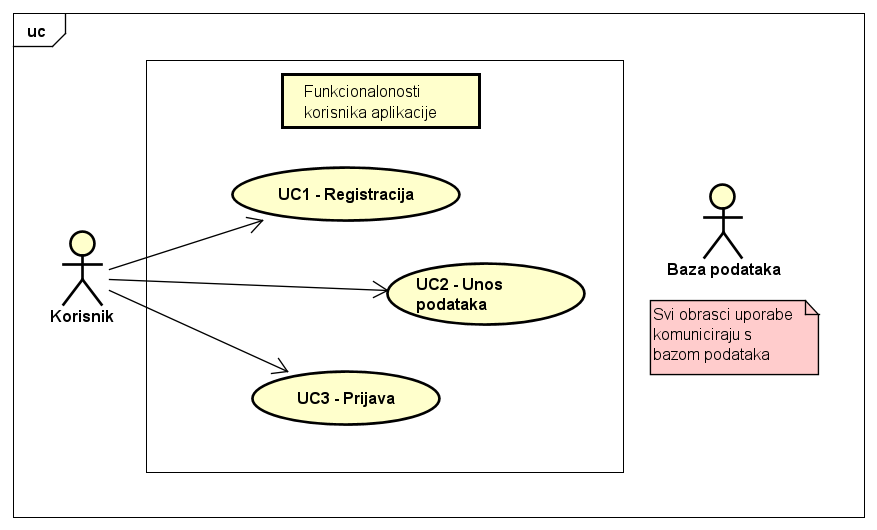
\includegraphics[scale=0.68]{dijagrami/UML_kor.PNG}
						\centering
						\caption{Dijagram obrasca uporabe, funkcionalnost korisnika}
						\label{fig:UML_kor}
					\end{figure}
				\eject
					
					\begin{figure}[h]
						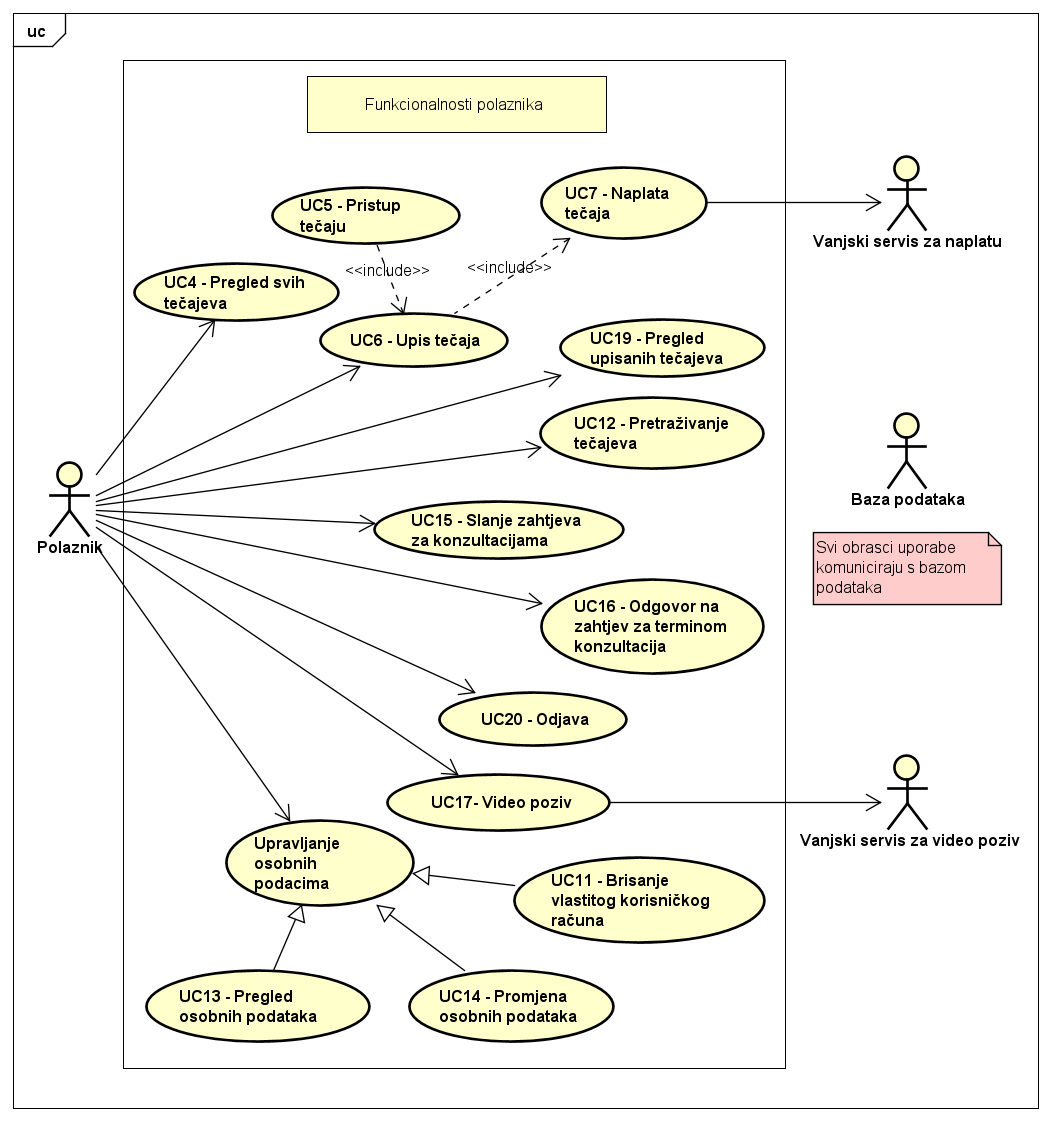
\includegraphics[scale=0.6]{dijagrami/UML_pol.PNG}
						\centering
						\caption{Dijagram obrasca uporabe, funkcionalnost polaznika tečaja}
						\label{fig:UML_pol}
					\end{figure}
				\eject
				
					\begin{figure}[h]
						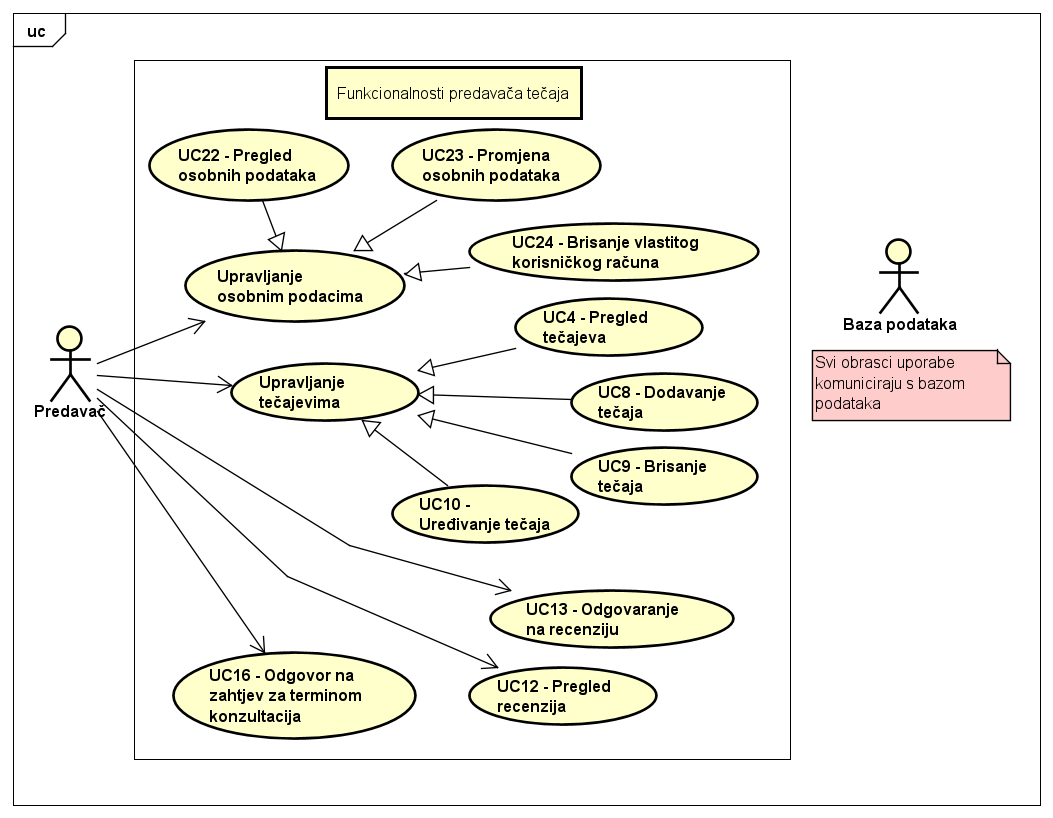
\includegraphics[scale=0.6]{dijagrami/UML_pred.PNG}
						\centering
						\caption{Dijagram obrasca uporabe, funkcionalnost predavača}
						\label{fig:UML_pred}
					\end{figure}
				\eject	
					\begin{figure}[h]
						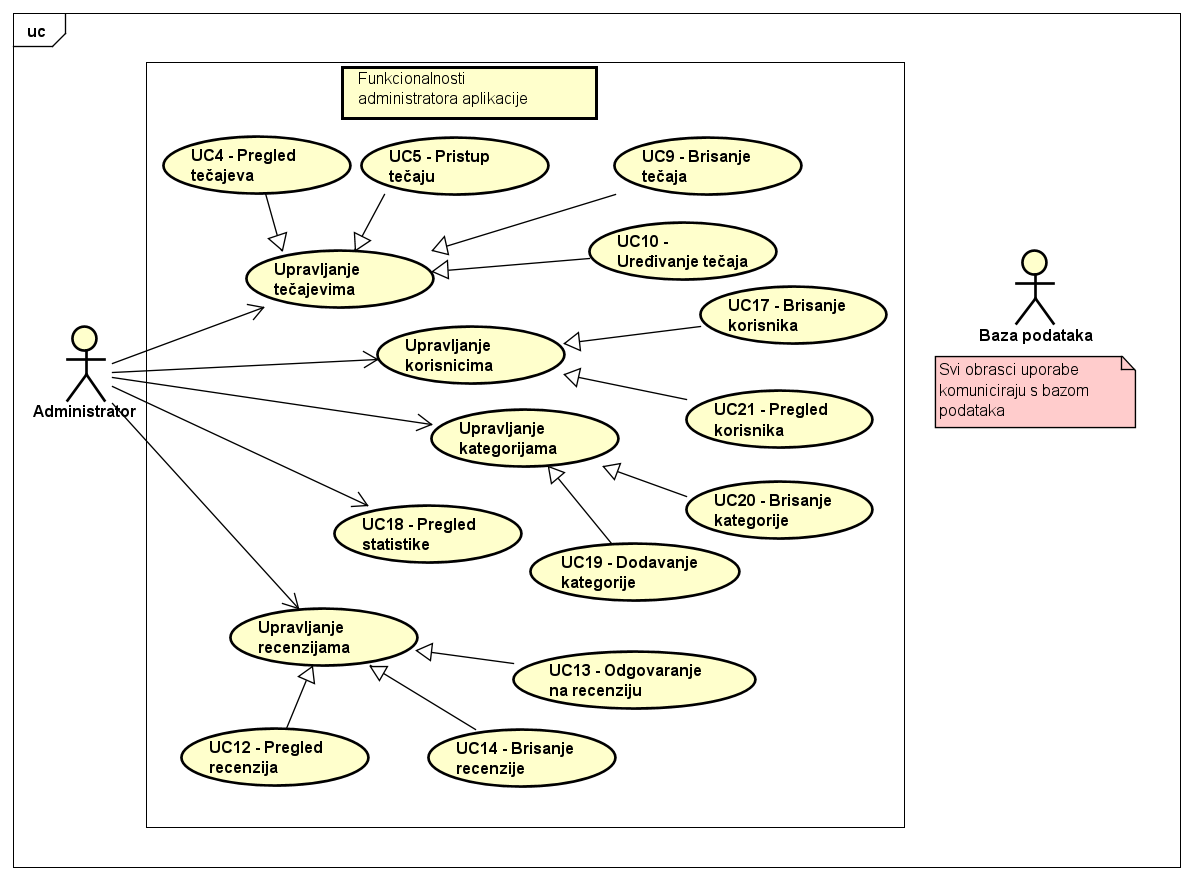
\includegraphics[scale=0.5]{dijagrami/UML_ad.PNG}
						\centering
						\caption{Dijagram obrasca uporabe, funkcionalnost administratora aplikacije}
						\label{fig:UML_ad}
					\end{figure}
				\eject		
				
			\subsection{Sekvencijski dijagrami}
				
				\textbf{\textit{dio 1. revizije}}\\
				
				\textit{Nacrtati sekvencijske dijagrame koji modeliraju najvažnije dijelove sustava (max. 4 dijagrama). Ukoliko postoji nedoumica oko odabira, razjasniti s asistentom. Uz svaki dijagram napisati detaljni opis dijagrama.}
				\eject
	
		\section{Ostali zahtjevi}
		
			\begin{packed_item}
				\item Sustav treba podržavati rad više korisnika u isto vrijeme
				\item Sustav treba biti jednostavan za korištenje, korisnici se moraju znati koristiti sučeljem bez opširnih uputa
				\item Neispravno korištenje sučelja ne smije narušiti funkcionalnost i rad sustava
				\item Sustav kao valutu koristi HRK
				\item Nadogradnja sustava ne smije narušavati postojeće funkcionalnosti sustava
				\item Korisničko sučelje i sustav moraju podržavati hrvatsku abecedu (dijakritičke znakove) pri unosu i prikazu tekstualnog sadržaja
				\item Veza s bazom podataka mora biti kvalitetno zaštićena, brza i otporna na vanjske greške
				\item Aplikacija mora imati responzivno korisničko sučelje
				\item Svi osobni podaci u aplikaciji moraju se čuvati u skladu s GDPR regulativom
			\end{packed_item}
			 
			 
			 
	